\documentclass[11pt,letterpaper,oneside]{article}

\title { Transcribiendo partituras a Clave de Fa }
\author{ Samuel Jos\'e Guti\'errez Avil\'es \\ \texttt{samaviles@gmail.com} }
\date{ Febrero 8, 2016 }

\usepackage{graphics}
\begin{document}

	\maketitle
  
	Lo primero que hay que hacer o pensar es que las claves son equivalentes,
	es decir con solo bajar una octava las notas tienen un lugar correspondientes
	en clave de Fa (Solo valido para trancibir partituras de clave de sol a clave de fa).\\
  
	Por ejemplo la nota do en la primera linea auxiliar en clave de sol:
	
	{%
\parindent 0pt
\noindent
\ifx\preLilyPondExample \undefined
\else
  \expandafter\preLilyPondExample
\fi
\def\lilypondbook{}%
\includegraphics{./4f/lily-bbba9c83-1}%
% eof

\ifx\postLilyPondExample \undefined
\else
  \expandafter\postLilyPondExample
\fi
}
  
	Es quivalente en clave de fa a:
  
	{%
\parindent 0pt
\noindent
\ifx\preLilyPondExample \undefined
\else
  \expandafter\preLilyPondExample
\fi
\def\lilypondbook{}%
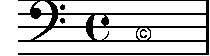
\includegraphics{./97/lily-ecfd06e8-1}%
% eof

\ifx\postLilyPondExample \undefined
\else
  \expandafter\postLilyPondExample
\fi
}\\
  
	Por tanto que:
  
	{%
\parindent 0pt
\noindent
\ifx\preLilyPondExample \undefined
\else
  \expandafter\preLilyPondExample
\fi
\def\lilypondbook{}%
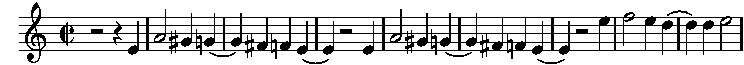
\includegraphics{./6c/lily-62e1cd08-1}%
% eof

\ifx\postLilyPondExample \undefined
\else
  \expandafter\postLilyPondExample
\fi
} ...
  
	Realizando la transposici\'on (bajando cada nota una octava), equivale en clave de fa a:
	
	{%
\parindent 0pt
\noindent
\ifx\preLilyPondExample \undefined
\else
  \expandafter\preLilyPondExample
\fi
\def\lilypondbook{}%
\includegraphics{./46/lily-441a9572-1}%
% eof

\ifx\postLilyPondExample \undefined
\else
  \expandafter\postLilyPondExample
\fi
} ...\\
	
	Lo siguiente a tener en cuenta es la tesitura del instrumento que interpretara
	la cancion pues hay situaciones en que las notas transportadas sobre pasan 
	el pentrama co clave de fa hacia abajo y son imposibles de tocar(En este 
	caso con fagot hay problema por amplia tesita del este instrumento).\\
  
	Tesitura del Fagot:
	
	{%
\parindent 0pt
\noindent
\ifx\preLilyPondExample \undefined
\else
  \expandafter\preLilyPondExample
\fi
\def\lilypondbook{}%
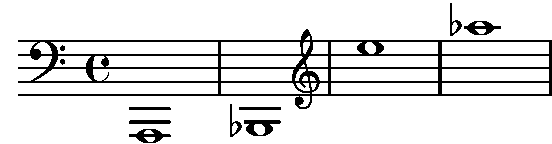
\includegraphics{./58/lily-9dd5db48-1}%
% eof

\ifx\postLilyPondExample \undefined
\else
  \expandafter\postLilyPondExample
\fi
}\\
  
	Por tanto con la simple transposici\'on seria suficiente para que las
	notas puedan ser ejecutadas (por el fagot) suponiendo que el interprete
	tenga dominio total del instrumento, por tanto lo otro que hay que tener
	en cuenta es que se busca que todas las notas no deben sobrepasar de
	la primera linea auxiliar inferior ni de la primera linea auxiliar superior
	mejorando la lectura de las mismas (las notas) y volviendose adecuadas
	para los instrumetos de tesitura grave.\\
	
	Rango de alturas para la escritura en clave de fa:
	
	{%
\parindent 0pt
\noindent
\ifx\preLilyPondExample \undefined
\else
  \expandafter\preLilyPondExample
\fi
\def\lilypondbook{}%
\includegraphics{./24/lily-4ba51b08-1}%
% eof

\ifx\postLilyPondExample \undefined
\else
  \expandafter\postLilyPondExample
\fi
} ...
	
	Esto provee de casi dos octavas (las octavas de basicas de casi todos)
	los instrumentos) para la colocacion de las notas.
	
	Por tanto:
	
	{%
\parindent 0pt
\noindent
\ifx\preLilyPondExample \undefined
\else
  \expandafter\preLilyPondExample
\fi
\def\lilypondbook{}%
\includegraphics{./46/lily-441a9572-1}%
% eof

\ifx\postLilyPondExample \undefined
\else
  \expandafter\postLilyPondExample
\fi
} ...
	
	Pasaria a ser:
	
	{%
\parindent 0pt
\noindent
\ifx\preLilyPondExample \undefined
\else
  \expandafter\preLilyPondExample
\fi
\def\lilypondbook{}%
\includegraphics{./a7/lily-6729e0ee-1}%
% eof

\ifx\postLilyPondExample \undefined
\else
  \expandafter\postLilyPondExample
\fi
} ...\\
	
	Todas las indicaciones anteriores validas en soniridad y tesituras de
	varios de los instrumentos graves (que se leen clave de fa). Tambi\'en
	lo que se busca en facilitar la lectura e interpretaci\'on, claro que 
	a medida que se va mejorando en la interpretaci\'on del instrumento
	vastara con una simple transposici\'on para mantener la integridad
	de la melodia.\\

\end{document} 
